\chapter{Parte 3}
\label{cap:p3}

\section{Análise do problema}

Na Parte II, a solução do modelo indica o tempo de inicio de cada atividade,
sabendo que todas as atividades demoram um certo tempo a serem executadas. Nesta parte assume-se
que é possível reduzir a duração de certas atividades a um dado custo
suplementar. Com isto pretende-se determinar quais as atividades em
que aplicar reduções de tempo de modo a que a realização do projeto seja
efetuada numa duração menor em 3 unidades de tempo relativamente ao previsto na Parte I e Parte II, com um custo suplementar mínimo possível. 


\section{Modelo}

\subsection{Parâmetros}

À semelhança da Parte I e Parte II, também aqui se tem como parâmetros do problema
a duração de cada atividade e as suas precedências. Os novos parâmetros são os
custos suplementares de redução de cada atividade e a quantidade máxima de
redução permitida para cada uma, em unidades de tempo.

Embora os custos normais das atividades sejam um parâmetro do problema, ele não foi considerado na construção do modelo visto o objetivo deste problema ser o de decidir que reduções de tempo se aplicam às atividades, a um custo suplementar mínimo. Os únicos custos relevantes neste contexto são por isso os custos suplementar de redução apenas, não sendo necessário considerar os custos normais de cada atividade na construção do modelo. Os custos normais da atividade foram apenas considerados na análise dos resultados para o cálculo do custo total do projeto (ver secção \ref{p3:resultado}).

\subsection{Variáveis de decisão}
\label{p3:vardec}
O modelo desta parte pretende reduzir o tempo de execução do
projeto da Parte I em 3 unidades de tempo. Para isso, assume-se que é possível aplicar unidades de redução à duração das atividades, com um custo suplementar associado. É importante saber que reduções se deve aplicar e em que atividades. Por isso, tem-se como variáveis de decisão
a redução (em unidades de tempo) a aplicar a cada umas das atividades. Essas reduções serão representadas por $R_{i}$. Por exemplo, $R_{5}$ representa a redução de tempo efetuada à atividade 5. Tal como nas partes anteriores, nodos finais e iniciais foram considerados como atividades ``fictícias'', existindo por isso as variáveis $R_{ini}$ e $R_{fim}$.

Neste modelo, como a duração de cada atividade pode ser reduzida, o tempo de início das atividades pode também ser alterado. Assim, além das variáveis de decisão apresentadas anteriormente, manteve-se as mesmas variáveis correspondentes aos tempos iniciais das atividades usadas na resolução do modelo da Parte II.
Decidiu-se também manter a mesma nomenclatura para essas variáveis: $T_{i}$.


\subsection{Função Objetivo}

Sabendo que o objetivo deste modelo é saber quais as atividades em que se deve
reduzir o tempo de duração, a um determinado custo suplementar, a função objetivo deverá ser uma expressão que indique o custo suplementar total inerente à redução de tempos aplicados a estas atividades. Este custo deve tomar o menor valor possível. Trata-se por isso de um problema de minimização. 

Os valores das variáveis de decisão $R_{i}$ indicam a redução (em unidades de tempo) que a atividade $i$ sofreu. Cada atividade tem um custo suplementar de redução associado, por unidade de tempo. Saber o custo suplementar das reduções aplicadas a uma atividade corresponde a multiplicar as unidades de tempo da redução pelo custo suplementar unitário de redução associado a essa atividade. Ou seja, o custo suplementar das reduções à duração de uma atividade, $Cr_{i}$ é dado por:

\begin{displaymath}
Cr_{i} = R_{i} \times C_{i}
\end{displaymath}

Onde:

\begin{itemize}
	\item[$R_{i}$] Variável de decisão, indica a redução (em unidades de tempo) aplicada à atividade $i$
	\item[$C_{i}$] Parâmetro do problema, indica o custo de redução (por unidade de tempo) associado à atividade $i$
\end{itemize}

O custo suplementar de redução do projeto todo será o somatório dos custos suplementares de cada atividade. Ou seja, a função objetivo, $z$, pode ser escrita de forma genérica como:

\begin{displaymath}
 min~z = \sum Cr_{i}
\end{displaymath}

Substituindo na fórmula os custos unitários de redução dados no enunciado, fica-se com a seguinte função objetivo:

\begin{displaymath} 
	\min~z = 100~R0 + 300~R1 + 100~R3 + 400~R4 + 800~R5 + 90~R6
	+ 500~R10 + 300~R11 
\end{displaymath}


\subsection{Restrições}

Com as restrições pretende-se indicar o espaço de possíveis soluções. Em primeiro lugar, sabe-se que há limites relativamente às unidades de tempo para as redução à duração que cada atividade pode sofrer. Assim, cada variável de decisão do modelo terá um limite superior. Conforme visto anteriormente, tem-se uma variável de decisão correspondente às unidades de tempo reduzidas em cada atividade. Cada atividade $i$, gera por isso uma restrição do tipo:

\begin{displaymath}
	 R_{i} \leq M_{i}
\end{displaymath}

Onde:
\begin{description}
	\item[$R_{i}$] Variável de decisão que indica a redução (em unidades de tempo)
		aplicada à atividade i.
	\item[$M_{i}$]Valor máximo de redução que é possível aplicar à atividade i
\end{description}

Analisando as reduções de tempo máximas permitidas para cada atividade, vemos que a atividade zero só pode
ser reduzida em 1 unidade de tempo, por exemplo, enquanto que as atividades
7 e 9 não podem ser reduzidas em nenhuma unidade de tempo, pois o valor máximo
de redução é zero. Traduzindo esta informação em termos matemáticos temos que
$R_{0} \leq 2$,  $R_{7} \leq 0$ e $R_{9} \leq 0$. A excepção à regra são as atividades finais e iniciais, que por serem atividades ``fictícias'' não irão ter qualquer redução de tempo, não gerando por isso nenhuma restrição deste tipo.

Em segundo lugar, tem-se restrições relativamente aos tempos de inicio de cada atividade,
semelhantes às da Parte II.\ Relembrando as restrições da parte
II:

\begin{displaymath} T_{i} \geq T_{j} + D_{j} \end{displaymath}

Sendo a atividade $i$ realizada após a atividade $j$, esta expressão indica que tempo de inicio da atividade $i$ tem obrigatoriamente de
ser maior ou igual à soma do tempo de inicio da atividade $j$ com a duração da
atividade $j$ pois é a atividade $j$ que precede à atividade $i$. Por exemplo,
sendo a atividade 0 aquela que precede a atividade 1, tínhamos que: 

\begin{displaymath} T_1 \ge T_0 + D_0 \Leftrightarrow T_1 \ge T_0
	+ 4 \end{displaymath}

A diferença neste modelo é que a duração da atividade precedente, a atividade $j$, pode ter sofrido
ou não uma redução no seu tempo de duração. Assim, na expressão é necessário subtrair a redução de tempo à duração inicial da atividade. Fica-se com:
\begin{displaymath}
T_{i} \ge T_{j} + (D_{j} - R{j})
\end{displaymath}

Onde:

\begin{itemize}
	\item[$T_{i}$] Tempo em que a atividade $i$ inicia
	\item[$T_{j}$] Tempo em que a atividade $j$ inicia
	\item[$D_{j}$] Duração da atividade $j$
	\item[$R_{j}$] Redução de tempo a aplicar na atividade $j$
\end{itemize}

Existe uma restrição deste tipo para cada uma das atividades existentes. 

Por último, tem-se uma restrição para forçar o tempo do projeto. Sabe-se que o tempo de inicio da atividade final corresponde à duração do projeto (visto na Parte II). Neste modelo, pretende-se reduzir a duração do projeto em 3 unidades de tempo relativamente ao tempo obtido na Parte I e Parte II. A duração do projeto nessas partes foi de 26 unidades de tempo. Pretende-se por isso que a nova duração seja de $26-3=23$ unidades de tempo. A duração total do projeto é dada por $T_{fim}$, tempo inicial da atividade final. Assim, forçar a que o projeto tenha uma duração específica corresponde a forçar essa variável a ter o valor de duração pretendido. Por esse motivo, no modelo tem-se a restrição:

\begin{displaymath}
T_{fim} = 23.
\end{displaymath}

Visto que os tempos e as reduções não podem ser negativos, neste modelo tem-se ainda restrições de não-negatividade:

\begin{displaymath}
T_{i} \geq 0; R_{i} \geq 0, \forall i_{\in\{ini, 0, 1, 3, 4,5,6,7,9,10,11,fim\}}
\end{displaymath}


\section{Ficheiro de \emph{input}}

O ficheiro de \emph{input} é constituído pela função objetivo e restrições,
detalhadas em secções anteriores.

\begin{verbatim}

=== FUNCAO OBJECTIVO ===

min: 100 R0 + 300 R1 + 100 R3 + 
		400 R4 + 800 R5 + 90 R6 + 500 R10 + 300 R11;

=== RESTRICOES ===

//Nodo inicial
Rini = 0;

//Nodo 0
R0 <= 1;
//Nodo 1
R1 <= 2;
//Nodo 3
R3 <= 1;
//Nodo 4
R4 <= 3;
//Nodo 5
R5 <= 1;
//Nodo 6
R6 <= 2;
//Nodo 7
R7 <= 0;
//Nodo 9
R9 <= 0;
//Nodo 10
R10 <= 1;
//Nodo 11
R11 <= 2;
//Nodo final
Rfim <= 0;

//Nodo Inicial
Tini >= 0 + 0;
//Nodo 0
T0 >= Tini + 0 - Rini;
//Nodo 1
T1 >= T0 + 4 - R0;
//Nodo 3
T3 >= T1 + 6 - R1;
T3 >= T5 + 4 - R5;
T3 >= T4 + 9 - R4;
//Nodo 4
T4 >= T0 + 4 - R0;
T4 >= T7 + 6 - R7;
//Nodo 5
T5 >= T4 + 9 - R4;
T5 >= T7 + 6 - R7;
T5 >= T10 + 8 - R10;
//Nodo 6
T6 >= Tini + 0 - Rini;
//Nodo 7
T7 >= T6 + 5 - R6;
//Nodo 9
T9 >= T7 + 6 - R7;
T9 >= T11 + 7 - R11;
T9 >= T10 + 8 - R10;
//Nodo 10
T10 >= T6 + 5 - R6;
//Nodo 11
T11 >= T10 + 8 - R10;
//Nodo final
Tfim >= T3 + 2 - R3;
Tfim >= T5 + 4 - R5;
Tfim >= T9 + 2 - R9;

Tfim = 26-3;

\end{verbatim}

\section{\emph{Output} produzido pelo \texttt{lp\_solve}}

O output apresentado a seguir foi obtido por \emph{copy-paste} direto resultante da execução do \emph{lp\_solve} num sistema linux para o ficheiro de input apresentado anteriormente:

\begin{verbatim}

Value of objective function: 280

Actual values of the variables:
R0                              0
R1                              0
R3                              1
R4                              0
R5                              0
R6                              2
R7                              0
R9                              0
R10                             0
R11                             0
Rini                            0
Rfim                            0
Tini                            0
T0                              0
T1                              4
T3                             22
T5                             18
T4                              9
T7                              3
T10                             3
T6                              0
T9                             18
T11                            11
Tfim                           23

Actual values of the constraints:
R1                              0
R2                              4
R3                             18
R4                              4
R5                             13
R6                              9
R7                              6
R8                              9
R9                             15
R10                            15
R11                             0
R12                             5
R13                            15
R14                             7
R15                            15
R16                             5
R17                             8
R18                             2
R19                             5
R20                             5

\end{verbatim}

\newpage
\section{Resultado}
\label{p3:resultado}

Os resultados do lpsolve mostram que se consegue reduzir a duração total do projeto em 3 unidades de tempo, passando o projeto a demorar 23 unidades de tempo, com um custo suplementar de 280 unidades monetárias. 

O custo total do projeto é dado pela soma dos custos normais das atividades com os custos suplementares de redução às suas durações, sendo este último valor o resultado obtido na função objetivo.

O custo normal das atividades é um parâmetro do problema. Somando o custo normal de todas as atividades temos:

\begin{displaymath}
800 + 900 + 2000 + 1000 + 300 = 5000~u.m.
\end{displaymath}

O custo total do projeto é por isso $5000 + 280 = 5280~u.m.$.

Na figura \ref{p3:fig:caminho_critico_sem_red} mostra-se o caminho crítico obtido bem como as durações das atividades da Parte I.

\begin{figure}[H]
	\centering
	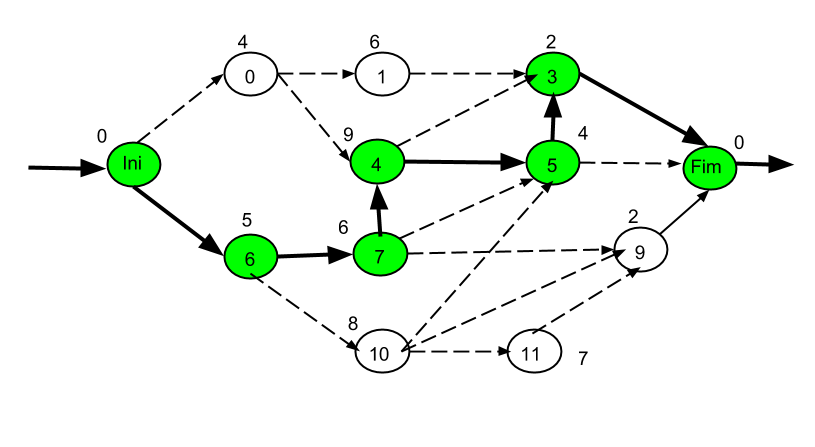
\includegraphics[scale=0.5]{./img/p1_caminho_critico}
	\caption{Grafo da Parte I, com indicação do caminho crítico e duração (em unidades de tempo) de cada atividade}
	\label{p3:fig:caminho_critico_sem_red}
\end{figure}

Agora a duração da atividade 3 é menor em 1 unidade, redução que custa 100 unidades monetárias, e a duração da atividade 6 é menor em duas unidades, redução que custa 180 unidades monetárias, tal como revelado no resultado \emph{output} do \texttt{lp\_solve}. Na figura \ref{p3:fig:caminho_critico_com_red} encontram-se representadas essas reduções.

\begin{figure}[H]
	\centering
	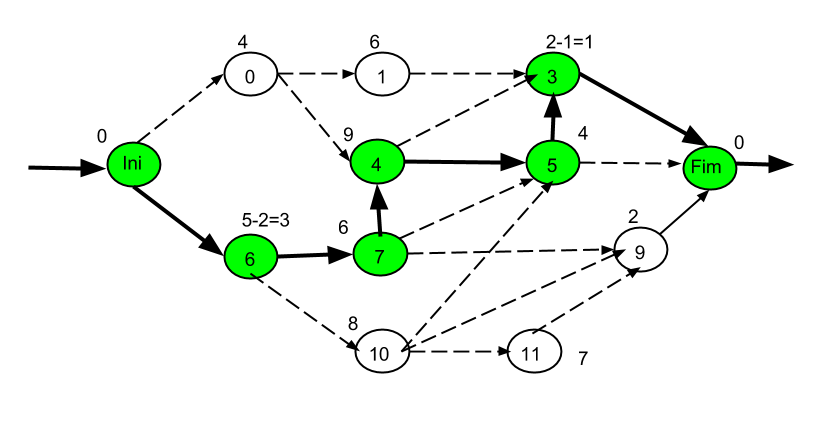
\includegraphics[scale=0.5]{./img/p3_caminho_critico_com_red}
	\caption{Grafo da parte I com as novas durações de cada atividade}
	\label{p3:fig:caminho_critico_com_red}
\end{figure}
 
Como se obteve reduções de tempo em atividades pertencentes ao caminho crítico da Parte I, conclui-se a solução do modelo da Parte I é única, e que por isso só existia um caminho crítico na rede. 
Além disso, somando as novas durações das atividades do caminho crítico da Parte I, vemos que o caminho tem a duração de 23 unidades de tempo e o resultado do modelo indica também uma duração total do projeto de 23 unidades de tempo. Ou seja, o caminho crítico da Parte I também continua a ser caminho crítico neste modelo, embora não haja a garantia que seja único.

A figura \ref{p3:fig:diagrama_gantt} representa o Diagrama de Gantt de acordo com os resultados do modelo. As
atividades que sofreram uma redução de tempo estão representadas a amarelo enquanto
que as atividades cuja duração não se alterou estão representadas a verde.
O caminho crítico está apresentado com preenchimento padrão preto.

\begin{figure}[H]
	\centering
	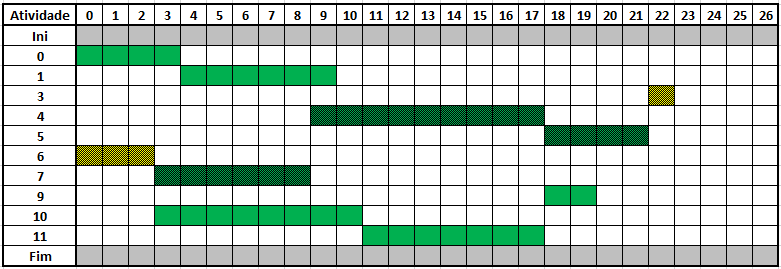
\includegraphics[scale=0.5]{./img/p3_diagrama_gantt}
	\caption{Diagrama de \emph{Gantt} com indicação do caminho crítico}
\label{p3:fig:diagrama_gantt}
\end{figure}


\section{Validação do modelo}

Para validar os resultados, tanto na função objetivo como nas restrições,
substituímos os valores das variáveis de decisão pelo valor que estas tomam na
solução que o \texttt{lp\_solve} indica como ótima. A ideia é verificar que os valores das
variáveis de decisão obtidos confirmam o valor da função objetivo obedecendo
a todas as restrições.

Para evitar ao máximo o erro humano, a substituição de variáveis foi feita
recorrendo a ferramentas que auxiliaram a substituição automática das variáveis
pelo seu valor.


\subsection{Variáveis de decisão}

No resultado obtido, todas as variáveis tomam um valor maior ou igual a 0, tal
como seria de esperar.

\subsection{Função objetivo}

Após a substituição das variáveis pelo valor obtido na solução, a função
objetivo fica:\\[0.5cm]

$100 * 0 + 300 * 0 + 100 *1 + 400 * 0 + 800 *0 + 90 *2
+ 500 *0 + 300 *0 = 100 * 1 + 90 * 2 = 280$\\[0.2cm]

Logo confirma-se que o custo total suplementar é de 280 unidades monetárias, tal como indica
a solução obtida com o \textit{lp\_solve}.\\[0.5cm]

\subsection{Restrições}

\begin{verbatim}
//Nodo inicial
Rini = 0;
0 = 0;

//Nodo 0
R0 <= 1;
0 <= 1;

//Nodo 1
R1 <= 2;
0 <= 2;

//Nodo 3
R3 <= 1;
1 <= 1;

//Nodo 4
R4 <= 3;
0 <= 3;

//Nodo 5
R5 <= 1;
0 <= 1;

//Nodo 6
R6 <= 2;
2 <= 2;

//Nodo 7
R7 <= 0;
0 <= 0;

//Nodo 9
R9 <= 0;
0 <= 0;

//Nodo 10
R10 <= 1;
0 <= 1;

//Nodo 11
R11 <= 2;
1 <= 2;

//Nodo final
Rfim <= 0;
0 <= 0;


//Nodo Inicial
Tini >= 0 + 0;
0 >= 0 + 0;

//Nodo 0
T0 >= Tini + 0 - Rini;
0 >= 0 + 0 - 0;

//Nodo 1
T1 >= T0 + 4 - R0;
4 >= 0 + 4 - 0;

//Nodo 3
T3 >= T1 + 6 - R1;
22 >= 4 + 6 - 0;

T3 >= T5 + 4 - R5;
22 >= 18 + 4 - 0;

T3 >= T4 + 9 - R4;
22 >= 9 + 9 - 0;

//Nodo 4
T4 >= T0 + 4 - R0;
9 >= 0 + 4 - 0;

T4 >= T7 + 6 - R7;
9 >= 3 + 6 - 0;

//Nodo 5
T5 >= T4 + 9 - R4;
18 >= 9 + 9 - 0;

T5 >= T7 + 6 - R7;
18 >= 3 + 6 - 0;

T5 >= T10 + 8 - R10;
18 >= 40 + 8 - 0;

//Nodo 6
T6 >= Tini + 0 - Rini;
0 >= 0 + 0 - 0;

//Nodo 7
T7 >= T6 + 5 - R6;
3 >= 0 + 5 - 2;

//Nodo 9
T9 >= T7 + 6 - R7;
18 >= 3 + 6 - 0;

T9 >= T11 + 7 - R11;
18 >= 41 + 7 - 1;

T9 >= T10 + 8 - R10;
18 >= 40 + 8 - 0;

//Nodo 10
T10 >= T6 + 5 - R6;
40 >= 0 + 5 - 2;

//Nodo 11
T11 >= T10 + 8 - R10;
41 >= 40 + 8 - 0;

//Nodo final
Tfim >= T3 + 2 - R3;
23 >= 22 + 2 - 1;

Tfim >= T5 + 4 - R5;
23 >= 18 + 4 - 0;

Tfim >= T9 + 2 - R9;
23 >= 18 + 2 - 0;

Tfim = 23;
23 = 23;


\end{verbatim}

Assim conclui-se que todas as restrições são respeitadas.
